\section{Regression Results}
The first approach was to compare fitting a regression model against the feature space to a physics based \ac{EGM}.
Three models were fit to the data: 
an SVM regression model, a Naive Bayes regression model, and a simple linear regression model.
These models were trained against a reduced set of data shown in figure \ref{fig:trainset}, and validated against the rest of the world.

\begin{figure}[h]
    \centering
    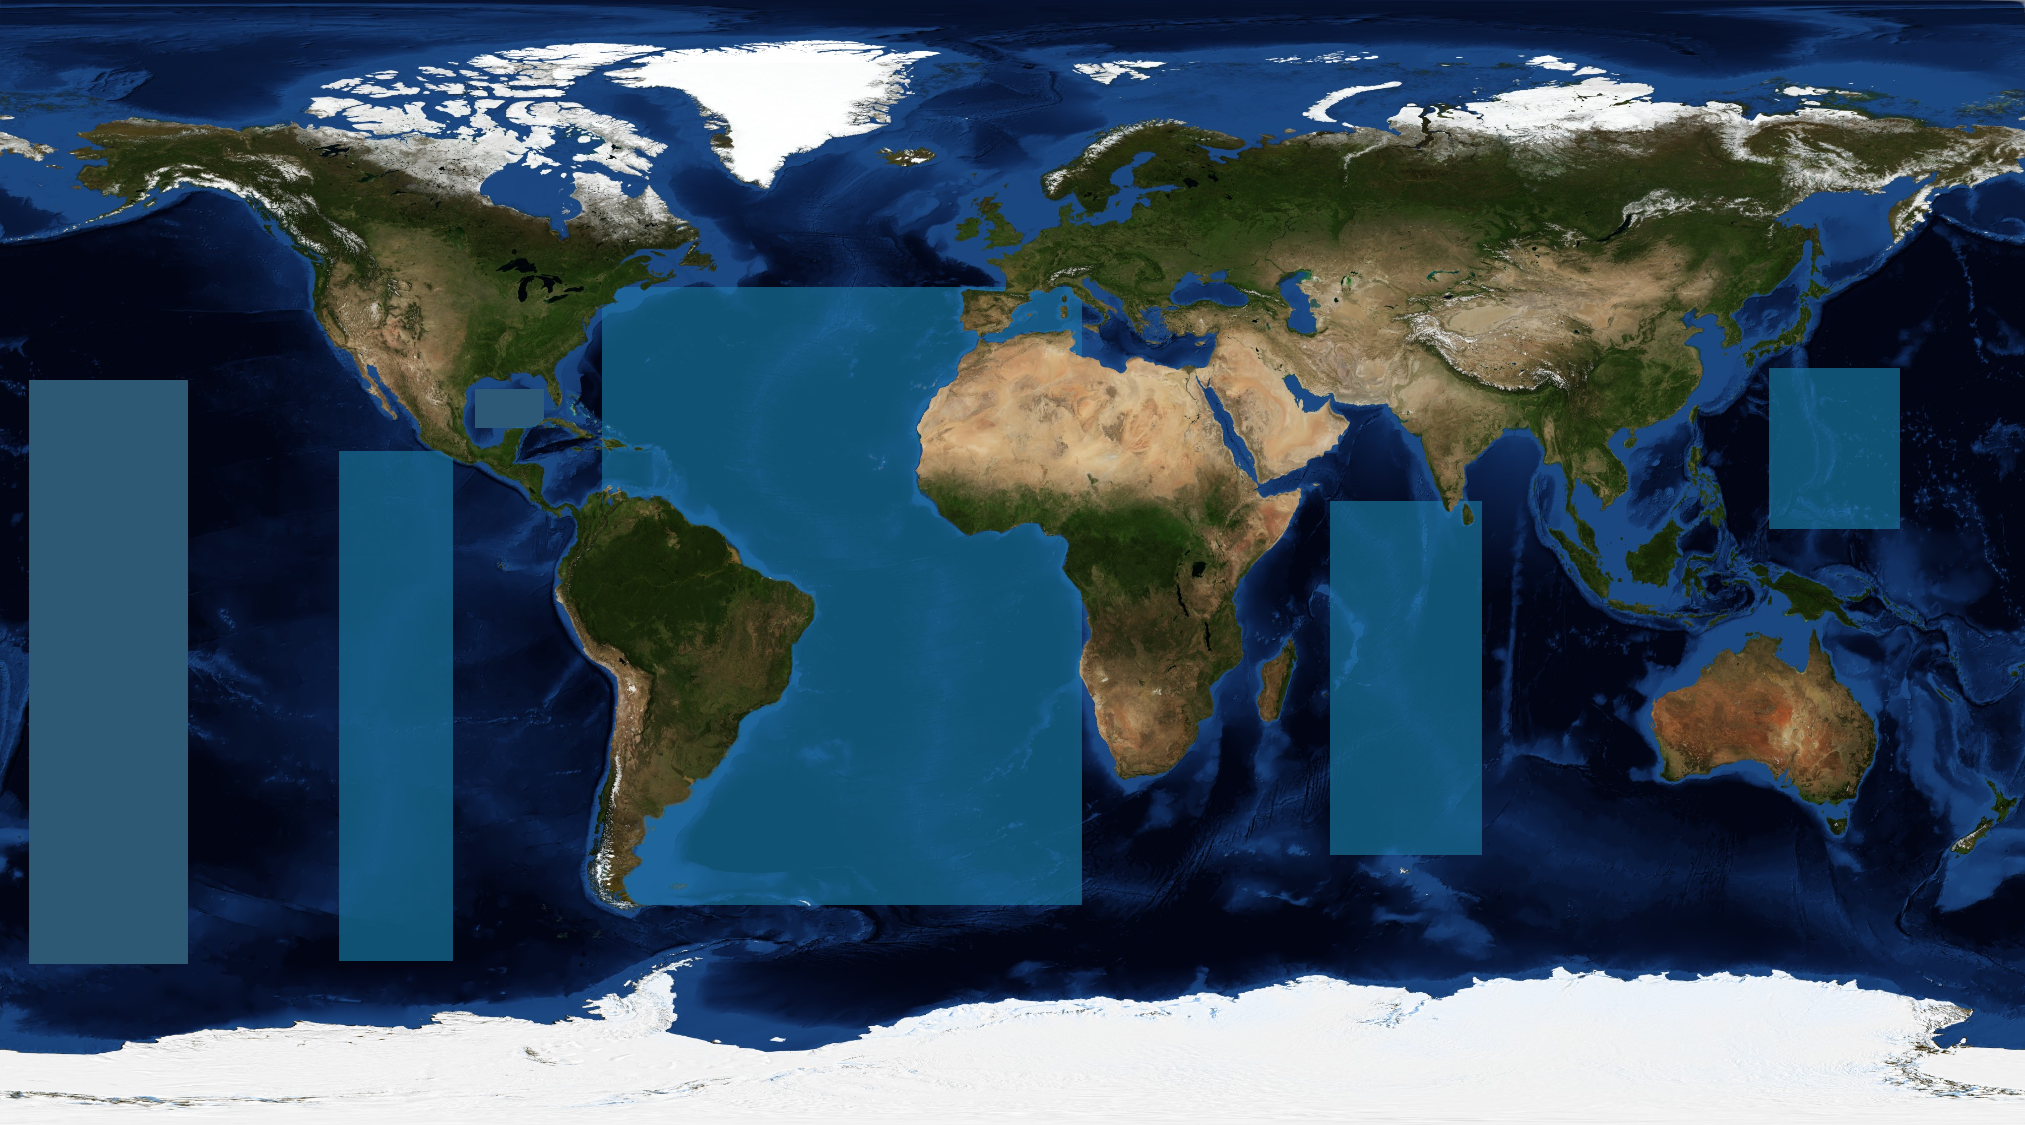
\includegraphics[width=\textwidth]{worldtraininglocal.png}
    \caption{Figure demonstrating initial training sets.}
    \label{fig:trainset}
\end{figure}

\begin{center}
    \begin{table}[htb]
        \begin{tabular}{|c c c|}
            \hline
				\textbf{Model} & \textbf{R Squared} & \textbf{RMSE} \\
				\hline
				SVM Regression & 0.841 & 365.23m \\
				Naive Bayes & 0.884 & 294.92m \\
				Linear Regression & 0.885 & 265.43m \\
				\hline
        \end{tabular}
        \label{table:REGRESSION_RESULTS}
        \caption{Regression Results}
    \end{table}
\end{center}

\subsection{Regression Results Discussion}
The regression model predictions under performed compared to existing \ac{EGM}s.
\cite{jena2012prediction} achieved a \ac{RMSE} of ~175m in their optimized model.
The linear regression model I fit in this work is 90m less accurate than the optimized model used in \cite{jena2012prediction}.
However, the R squared score is high for each model. 
This shows that the data correlates well and that a good model can fit the data well.
While the regression results were uninspiring, the R2 score shows that a model can potentially perform well.



%
%
%end{tabular}

% \begin{sidewaysfigure}[h]
%     \centering
%     \begin{tikzpicture}
%         \node[align=left,draw] 
% 		at ([yshift=-35pt]current bounding box.south)
% 		{%
% 			\begin{tabular}{c l c l c l c l}

% 				\begin{tikzpicture}
% 					\draw[fill opacity=0.5,fill=rfc] (0,0) rectangle (1,0.25);
% 				\end{tikzpicture}
% 				& RandonForestClassifier &  

% 				\begin{tikzpicture}
% 					\draw[fill opacity=0.5,fill=ada] (0,0) rectangle (1,0.25);
% 				\end{tikzpicture}
% 				& AdaBoostClassifier &

% 				\begin{tikzpicture}
% 					\draw[fill opacity=0.5,fill=grad] (0,0) rectangle (1,0.25);
% 				\end{tikzpicture}
%                 & GradientBoostingClassifier & 
% 				\begin{tikzpicture}
% 					\draw[fill opacity=0.5,fill=qda] (0,0) rectangle (1,0.25);
% 				\end{tikzpicture}
%                 & QDA \\ 
% 				\begin{tikzpicture}
% 					\draw[fill opacity=0.5,fill=dtc] (0,0) rectangle (1,0.25);
% 				\end{tikzpicture}
%                 & DecisionTree & 
% 				\begin{tikzpicture}
% 					\draw[fill opacity=0.5,fill=voting] (0,0) rectangle (1,0.25);
% 				\end{tikzpicture}
%                 & VotingClassifier & 

% 				\begin{tikzpicture}
% 					\draw[fill opacity=0.5,fill=bag] (0,0) rectangle (1,0.25);
% 				\end{tikzpicture}
%                 & Bagging &                
%                 \begin{tikzpicture}
% 					\draw[fill opacity=0.5,fill=mlp] (0,0) rectangle (1,0.25);
% 				\end{tikzpicture}
%                 & ANN \\
% 				\begin{tikzpicture}
% 					\draw[fill opacity=0.5,fill=knn] (0,0) rectangle (1,0.25);
% 				\end{tikzpicture}
%                 & KNN &

% 				\begin{tikzpicture}
% 					\draw[fill opacity=0.5,fill=gau] (0,0) rectangle (1,0.25);
% 				\end{tikzpicture}
%                 & NaiveBayes &
%                 \begin{tikzpicture}
% 					\draw[fill opacity=0.5,fill=land] (0,0) rectangle (1,0.25);
% 				\end{tikzpicture}
%                 & LAND \\
% 			\end{tabular}
% 		};
%     \end{tikzpicture}
%     \caption{}
%     \label{}
% \end{sidewaysfigure}